\label{Jonas}
Um sich einen Überblick über die Thematik verschaffen zu können, wurden verschiedene Self-Assessment-Tests anderer Universitäten analysiert. Hierbei ist wichtig zu wissen, dass folgende Beschreibungen sich nur auf die jeweiligen \textit{Graphical User Interfaces} der Tests beziehen und es generell nicht möglich ist, auf die Implementierung, die dahinter steckt, genauer einzugehen.
\subsection{Test der Universität Frankfurt}
Der Test beginnt mit einem Motivationstext, der sowohl Sinn und Zweck des Tests erklärt, als auch den User in die Benutzung einführt. Dies wurde bei unserer Arbeit weggelassen, da eine Einführung auch auf der jeweiligen Webseite, die unseren Test integriert, hinzugefügt werden kann. Desweiteren wird angebote n den Test der Universität Frankfurt runterzuladen, was eine Offline-Ausarbeitung realisiert. Bei unserem Test wird der aktuelle Zustand in der URL der Webseite kodiert. Dies ermöglicht zwar keine Bearbeitung ohne Internet, bietet aber an, den Test jederzeit zu pausieren, indem man sich die URL rauskopiert. Der zu vergleichende Test erfordert außerdem eine persönliche Registrierung, welche sehr ausführlich ist, was dazu führt, dass die User Experience sinkt. Daher wurde eine Registrierung in unserem Test weggelassen, um die Flexibilität und Einfachheit zu gewährleisten. Eine weitere Einschränkung ist die Notwendigkeit des Adobe Flash Players, auf den wir ganz verzichten. 
\begin{figure}[htbp] 
  \centering
     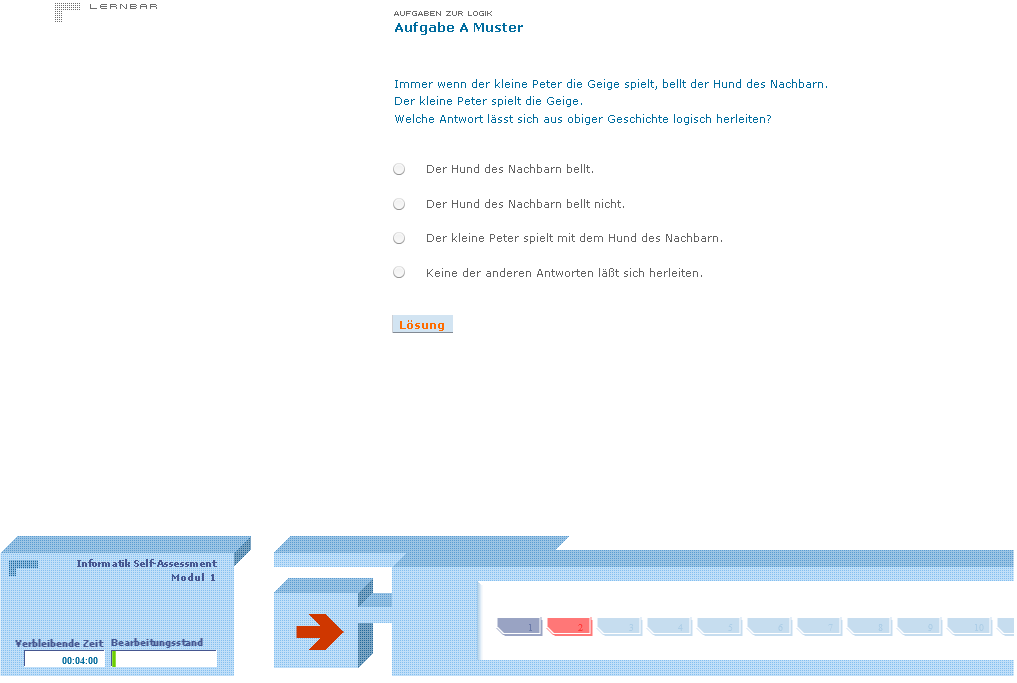
\includegraphics[width=0.5\textwidth]{Jonas_Images/frankfurt1.png}
  \caption{}
  \label{fig:Bild1}
\end{figure}
In Abbildung 1 ist das Grundlayout des Tests von der Universität Frankfurt zu sehen\cite{Frankfurt}. Das Layout ist sehr ähnlich zu unserem und weist die Frage mit ihren Antworten, einen Fortschrittsbalken, einen Next-Button und einer Zeitanzeige auf. Auch ist es möglich Grafiken anzeigen zu lassen. Der Test wird in verschiedene Kategorien eingegliedert, die wiederholbar sind. Bei unserem Test ist die Erstellung von Kategorien ebenfalls möglich, aber auf jegliche Wiederholungen wurden verzichtet.
\begin{figure}[htbp] 
  \centering
     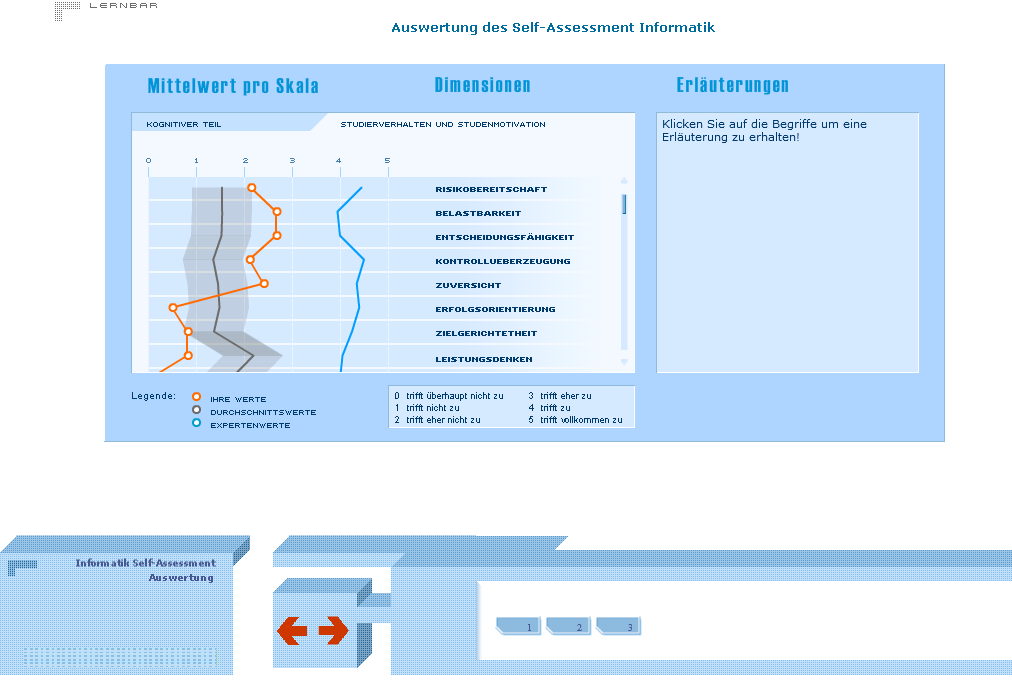
\includegraphics[width=0.5\textwidth]{Jonas_Images/frankfurt2.png}
  \caption{}
  \label{fig:Bild2}
\end{figure}
Abschließend bietet der Test der Universität Frankfurt eine Bewertung der beantworteten Fragen, die in Abbildung 2 zu sehen ist. Die Grafik ist zwar schön anzusehen, jedoch fehlt hier eine klare Interpretation der Ergebnisse: Das Endresultat muss man quasi selbst entscheiden. Daher haben wir bei unserem Test darauf geachtet, dass eine persönliche Beurteilung hinzugefügt werden kann, die zum Beispiel dem User Tipps gibt, falls er in einer Kategorie schlecht abschneidet oder setzt generell die Ergebnisse des Users in Bezug auf den Studiengang.
\subsection{Test der FU Berlin}
\begin{figure}[htbp] 
  \centering
     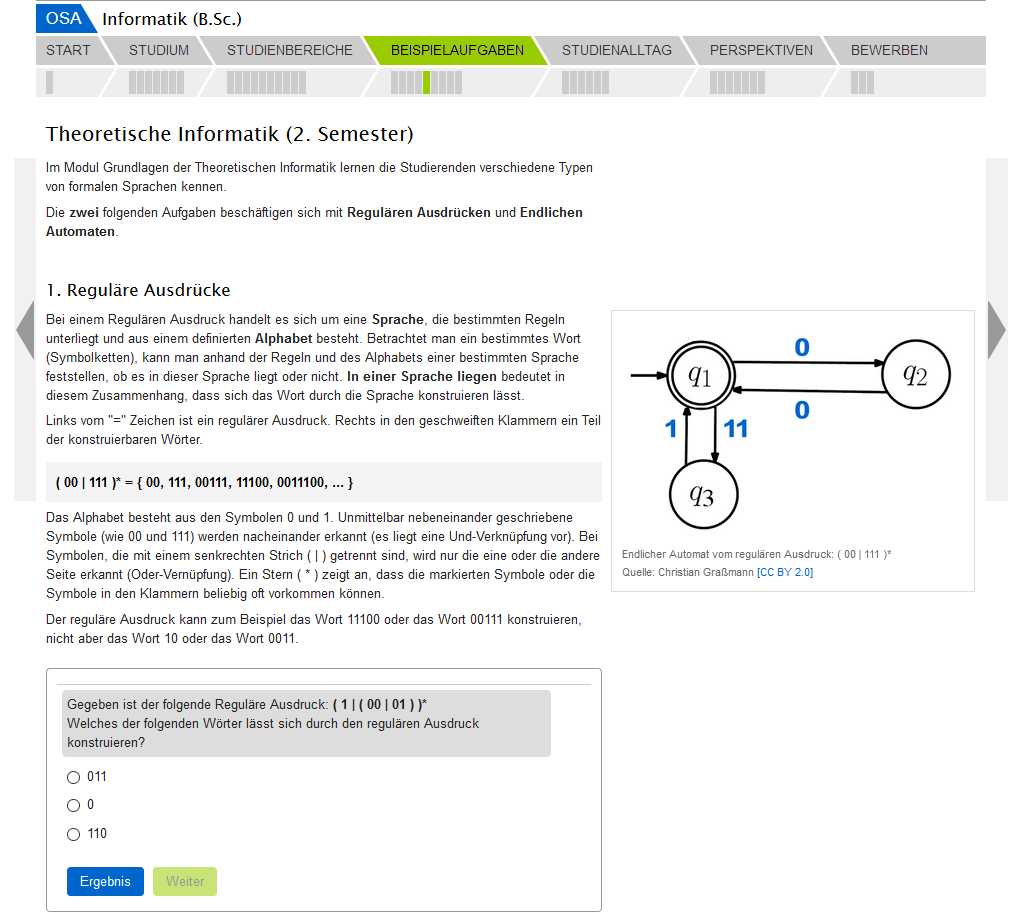
\includegraphics[width=0.5\textwidth]{Jonas_Images/berlin.png}
  \caption{}
  \label{fig:Bild3}
\end{figure}
Abbildung 3 zeigt einen Ausschnitt aus dem  Test der FU Berlin\cite{Berlin}. Dieser veranschaulicht eine schöne Gliederung und auch die Möglichkeit das Ergebnis der Frage sofort zu sehen. Hier wird viel mit Multimedia gearbeitet, was das Interesse der User fangen soll, um die User Experience zu steigern. Auch in unserem Test ist das einbetten von Multimedia-Dateien möglich.
\subsection{Test der RWT Aachen}
\begin{figure}[htbp] 
  \centering
     \includegraphics[width=0.5\textwidth]{Jonas_Images/abschnitte.png}
  \caption{}
  \label{fig:Bild4}
\end{figure}
Der Test der RWT Aachen ähnelt unserem Modell wie man in Abbildung 4 sehen kann\cite{Aachen}. Das Layout ist einfach gehalten und überschaubar. Es gibt einen Next-Button und einen Fortschrittsbalken. Allerdings bietet der Test keine Möglichkeit an, die Fragen zu überspringen, was bei unserem Test durchaus machbar ist. Auch bietet der Test der RWT Aachen keinen mobilen Support. Dies ist bei uns automatisch integriert, da wir mit dem Webbrowser arbeiten.